\section{Luthfi Muhammad Nabil/1174035}
\subsection{Soal 1}
Buatlah fungsi pada file chap4\_1174035\_csv.py untuk membuka file csv dengan lib csv mode list : 
\lstinputlisting[firstline=2, lastline=6]{src/4/1174035/Praktek/chap4_1174035_csv.py}

\subsection{Soal 2}
Buatlah fungsi pada file chap4\_1174035\_csv.py untuk membuka file csv dengan lib csv mode dictionary : 
\lstinputlisting[firstline=8, lastline=12]{src/4/1174035/Praktek/chap4_1174035_csv.py}

\subsection{Soal 3}
Buatlah fungsi pada file chap4\_1174035\_pandas.py untuk membuka file csv dengan lib pandas mode list : 
\lstinputlisting[firstline=2, lastline=5]{src/4/1174035/Praktek/chap4_1174035_pandas.py}

\subsection{Soal 4}
Buatlah fungsi pada file chap4\_1174035\_pandas.py untuk membuka file csv dengan lib pandas mode dictionary : 
\lstinputlisting[firstline=6, lastline=10]{src/4/1174035/Praktek/chap4_1174035_pandas.py}

\subsection{Soal 5}
Buatlah fungsi baru di chap4\_1174035\_pandas.py untuk mengubah format tanggal menjadi standard dataframe : 
\lstinputlisting[firstline=11, lastline=13]{src/4/1174035/Praktek/chap4_1174035_pandas.py}

\subsection{Soal 6}
Buatlah fungsi baru di chap4\_1174035\_pandas.py untuk mengubah index kolom : 
\lstinputlisting[firstline=14, lastline=16]{src/4/1174035/Praktek/chap4_1174035_pandas.py}

\subsection{Soal 7}
Buatlah fungsi baru di chap4\_1174035\_pandas.py untuk mengubah atribut atau nama kolom : 
\lstinputlisting[firstline=17, lastline=19]{src/4/1174035/Praktek/chap4_1174035_pandas.py}

\subsection{Soal 8}
Buatlah program chap4\_1174035\_main.py yang menggunakan library chap4\_1174035\_csv.py yang membuat dan membaca file CSV : 
\lstinputlisting{src/4/1174035/Praktek/chap4_1174035_main.py}

\subsection{Soal 9}
Buatlah program chap4\_1174035\_main2.py yang menggunakan library chap4\_1174035\_csv.py yang membuat dan membaca file CSV : 
\lstinputlisting{src/4/1174035/Praktek/chap4_1174035_main2.py}

\subsection{Penanganan Error}
Error yang didapat : KeyError
Deskripsi : Error saat kunci ada yang salah atau tidak ada di dalam file CSV 
\begin{figure}[!htbp]
	\centering
	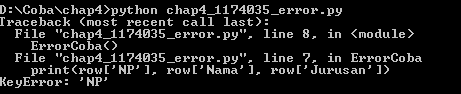
\includegraphics[height=4cm, width=10cm]{figures/4/1174035/Praktek/chap4_1174035_error.png}
	\caption{Contoh KeyError}
	\label{1174035_Error}
\end{figure}
Penanganan : Menggunakan KeyError seperti pada line berikut : \lstinputlisting{src/4/1174035/Praktek/chap4_1174035_error.py}
\begin{figure}[!htbp]
	\centering
	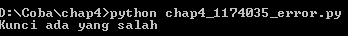
\includegraphics[height=4cm, width=10cm]{figures/4/1174035/Praktek/chap4_1174035_errorfix.png}
	\caption{Hasil Penanganan Error}
	\label{1174035_ErrorFix}
\end{figure}


\section{Irvan Rizkiansyah/1174043}
	\subsection{Soal 1}
		\lstinputlisting[firstline=10, lastline=14]{src/4/1174043/Praktek/chap4_1174043_csv.py}
	\subsection{Soal 2}
		\lstinputlisting[firstline=16, lastline=20]{src/4/1174043/Praktek/chap4_1174043_csv.py}
	\subsection{Soal 3}
		\lstinputlisting[firstline=10, lastline=12]{src/4/1174043/Praktek/chap4_1174043_pandas.py}
	\subsection{Soal 4}
		\lstinputlisting[firstline=14, lastline=17]{src/4/1174043/Praktek/chap4_1174043_pandas.py}
	\subsection{Soal 5}
		\lstinputlisting[firstline=19, lastline=21]{src/4/1174043/Praktek/chap4_1174043_pandas.py}
	\subsection{Soal 6}
		\lstinputlisting[firstline=23, lastline=26]{src/4/1174043/Praktek/chap4_1174043_pandas.py}
	\subsection{Soal 7}
		\lstinputlisting[firstline=28, lastline=31]{src/4/1174043/Praktek/chap4_1174043_pandas.py}
	\subsection{Soal 8}
		\lstinputlisting[firstline=8, lastline=12]{src/4/1174043/Praktek/chap4_1174043_main.py}
	\subsection{Soal 9}
		\lstinputlisting[firstline=8, lastline=14]{src/4/1174043/Praktek/chap4_1174043_main2.py}
	\subsection{Penanganan Error}
		\lstinputlisting[firstline=8, lastline=17]{src/4/1174043/Praktek/chap4_1174043_error.py}
		\begin{figure} [ht]
			\centerline{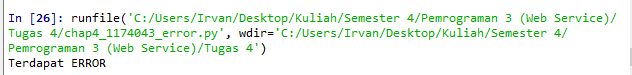
\includegraphics[width=0.6\textwidth]{figures/4/1174043/Praktek/fix_error.png}}
			\caption{Fix Error}
			\label{Fix Error}
		\end{figure}

		\ref{fix_error}

\section{Hagan Rowlenstino/1174040}
\subsection{Soal 1}
Buatlah fungsi untuk membuka file csv dengan lib csv mode list : 
\lstinputlisting{src/4/1174040/Praktek/1174040_CSV1.py}

\subsection{Soal 2}
Buatlah fungsi untuk membuka file csv dengan lib csv mode dictionary : 
\lstinputlisting{src/4/1174040/Praktek/1174040_CSV2.py}

\subsection{Soal 3}
Buatlah fungsi  untuk membuka file csv dengan lib pandas mode list : 
\lstinputlisting{src/4/1174040/Praktek/1174040_pandas1.py}

\subsection{Soal 4}
Buatlah fungsi  untuk membuka file csv dengan lib pandas mode dictionary : 
\lstinputlisting{src/4/1174040/Praktek/1174040_pandas2.py}

\subsection{Soal 5}
Buatlah fungsi untuk mengubah format tanggal menjadi standard dataframe : 
\lstinputlisting{src/4/1174040/Praktek/1174040_pandas3.py}

\subsection{Soal 6}
Buatlah fungsi  untuk mengubah index kolom : 
\lstinputlisting{src/4/1174040/Praktek/1174040_pandas4.py}

\subsection{Soal 7}
Buatlah fungsi  untuk mengubah atribut atau nama kolom : 
\lstinputlisting{src/4/1174040/Praktek/1174040_pandas5.py}

\subsection{Soal 8}
Disini saya telah membuat file CSV bernama 1174040\_csv.csv untuk di tampilkan, dan sebelum me write ke dalam file csv, terlebih dahulu buat file 1174040\_writecsv.csv : 
\lstinputlisting{src/4/1174040/Praktek/1174040_main.py}

\subsection{Soal 9}
Disini saya telah membuat file CSV bernama 1174040\_csvpandas.csv untuk ditampilkan, dan sebelum me write ke dalam file csv, telebih dahulu buat file 1174040\_writepandas.csv : 
\lstinputlisting{src/4/1174040/Praktek/1174040_main2.py}

\section{Faisal Najib Abdullah 1174042}
\subsection{Praktek}
\begin{enumerate}
	\item Buatlah  fungsi  (file  terpisah/library  dengan  nama  NPMcsv.py)  untuk  membuka file csv dengan lib csv mode list.
	
	\lstinputlisting[caption = Fungsi untuk membuka file CSV dengan lib CSV mode list., firstline=10, lastline=15]{src/4/1174042/Praktek/1174042csv.py}
	
	\item Buatlah  fungsi  (file  terpisah/library  dengan  nama  NPMcsv.py)  untuk  membuka file csv dengan lib csv mode dictionary.
	
	\lstinputlisting[caption =  Fungsi untuk membuka file CSV dengan lib CSV mode dictionary., firstline=17, lastline=22]{src/4/1174042/Praktek/1174042csv.py}
	
	\item Buatlah fungsi (file terpisah/library dengan nama NPMpandas.py) untuk membuka file csv dengan lib pandas mode list.
	
	\lstinputlisting[caption =  Fungsi untuk membuka file CSV dengan lib Pandas mode list., firstline=10, lastline=13]{src/4/1174042/Praktek/1174042pandas.py}
	
	\item Buatlah fungsi (file terpisah/library dengan nama NPMpandas.py) untuk membuka file csv dengan lib pandas mode dictionary.
	
	\lstinputlisting[caption =  Fungsi untuk membuka file CSV dengan lib Pandas mode dictionary., firstline=10, lastline=13]{src/4/1174042/Praktek/1174042pandas.py}
	
	\item  Buat fungsi baru di NPMpandas.py untuk mengubah format tanggal menjadi standar dataframe.
	
	\lstinputlisting[caption =  Fungsi untuk mengubah format tanggal menjadi standar dataframe., firstline=15, lastline=19]{src/4/1174042/Praktek/1174042pandas.py}
	
	\item Buat fungsi baru di NPMpandas.py untuk mengubah index kolom.
	
	\lstinputlisting[caption =  Fungsi untuk mengubah index kolom., firstline=21, lastline=24]{src/4/1174042/Praktek/1174042pandas.py}
	
	\item Buat fungsi baru di NPMpandas.py untuk mengubah atribut atau nama kolom.
	
	\lstinputlisting[caption =  Fungsi untuk mengubah atribut atau nama kolom., firstline=26, lastline=30]{src/4/1174042/Praktek/1174042pandas.py}
	
	\item Buat program main.py yang menggunakan library NPMcsv.py yang membuat dan membaca file csv.
	
	\lstinputlisting[caption =  Membuat dan mebaca file CSV menggunakan library 1174006pandas., firstline=8, lastline=13]{src/4/1174042/Praktek/1174042main.py}
	
	\item Buat program main2.py yang menggunakan library NPMpandas.py yang membuat dan membaca file csv.
	
	\lstinputlisting[caption = Membuat dan mmebaca file CSV menggunakan library 1174006pandas., firstline=8, lastline=13]{src/4/1174042/Praktek/1174042main2.py}
	
\end{enumerate}

\subsection{Ketrampilan Penanganan Error}
Error yang di dapat dari mengerjakan tugas ini adalah type error, cara menaggulaginya dengan cara mengecheck kembali codingannya
kemudian run kembali aplikasinya
berikut contoh Penggunaan fungsi try dan exception
\lstinputlisting{src/4/1174042/Praktek/1174042_2err.py}

